%
% domani.tex
%
% (c) 2019 Prof Dr Andreas Müller, Hochschule Rapperswil
%
\begin{frame}
\frametitle{Domain}

\def\s{0.7}
\begin{columns}[T,totalwidth=\linewidth]
\begin{column}{0.48\textwidth}
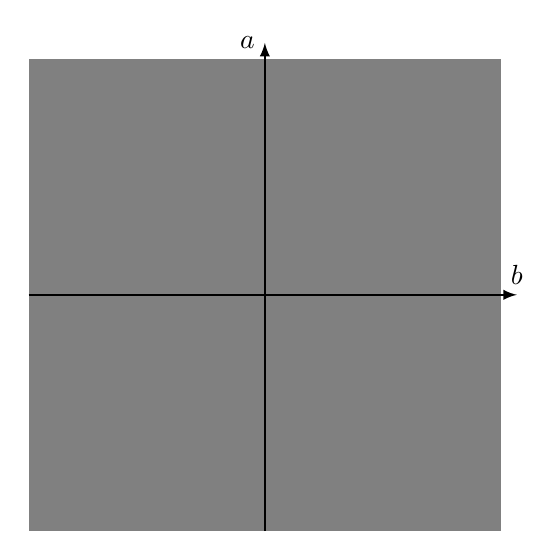
\begin{tikzpicture}[>=latex]
\begin{scope}
\clip (-3,-3) rectangle (3,3);
\fill[color=gray] (-3,-3) rectangle (3,3);
\end{scope}
\draw[->,line width=0.7pt] (-3,0)--(3.2,0) coordinate[label={$b$}];
\draw[->,line width=0.7pt] (0,-3)--(0,3.2) coordinate[label={left:$a$}];
\end{tikzpicture}
\end{column}
\begin{column}{0.48\textwidth}
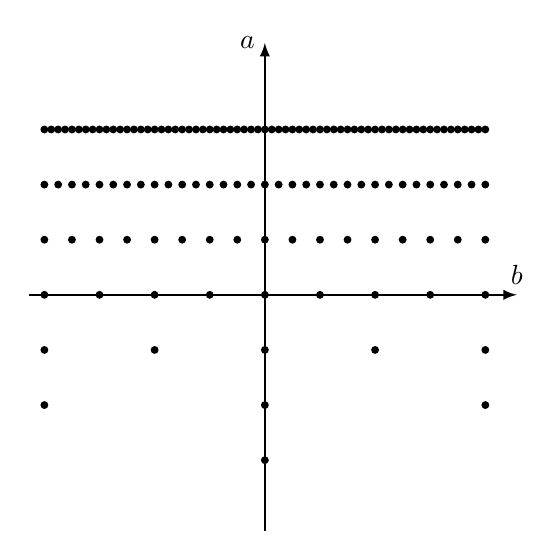
\begin{tikzpicture}[>=latex]
\begin{scope}
\clip (-3,-3) rectangle (3,3);
\foreach \x in {0}{
	\fill ({\x*\s},{-3*\s}) circle[radius=0.05];
}
\foreach \x in {-4,0,4}{
	\fill ({\x*\s},{-2*\s}) circle[radius=0.05];
}
\foreach \x in {-4,-2,...,4}{
	\fill ({\x*\s},{-1*\s}) circle[radius=0.05];
}
\foreach \x in {-4,...,4}{
	\fill ({\x*\s},{0*\s}) circle[radius=0.05];
}
\foreach \x in {-4,-3.5,...,4}{
	\fill ({\x*\s},{1*\s}) circle[radius=0.05];
}
\foreach \x in {-4,-3.75,...,4}{
	\fill ({\x*\s},{2*\s}) circle[radius=0.05];
}
\foreach \x in {-4,-3.875,...,4}{
	\fill ({\x*\s},{3*\s}) circle[radius=0.05];
}
\end{scope}
\draw[->,line width=0.7pt] (-3,0)--(3.2,0) coordinate[label={$b$}];
\draw[->,line width=0.7pt] (0,-3)--(0,3.2) coordinate[label={left:$a$}];
\end{tikzpicture}
\end{column}
\end{columns}

\end{frame}
